\chapter{ClamAV bytecode language}
The bytecode that ClamAV loads is a simplified form of the LLVM Intermediate Representation, and as such it is language-independent.

However currently the only supported language from which such bytecode can be
generated is a simplified form of C.

The ClamAV bytecode backend translates from LLVM IR to ClamAV bytecode.
Theoretically it could translate any LLVM IR which meets these constraints:
\begin{itemize}
\item No external function calls, except those defined by the ClamAV API
\item No inline assembly
\item ...
 %TODO: the constraints
\end{itemize}

Thus (theoretically) any language that doesn't need an external language runtime (or
the runtime can be compiled to the above restricted set of LLVM IR), could be
compiled to ClamAV bytecode.

There are currently no plans currently to support any other language than C (maybe C++ when
clang will support it).

\section{Predefines}
The following macros are predefined:
\lstset{basicstyle=\tiny}
\lstinputlisting{predefines}
\lstset{basicstyle=\footnotesize}

\section{ClamAV API header restrictions}
The ClamAV API header file (\verb+bytecode_api.h+, and any files included by it) must be both valid C code, and conform to the following BNF grammar:
%TODO: write the grammar here

The reason is that the \verb+ifacegen+ program must be able to parse it to
generate the api description, and glue code, and it only recognizes the above
BNF grammar.

This also adds portability checks: any code conforming to that grammar should
work properly both in the interpret and the JIT, even though a number of things
have changed (such as sizeof int, which is why only fixed-size integers are
allowed in the API).
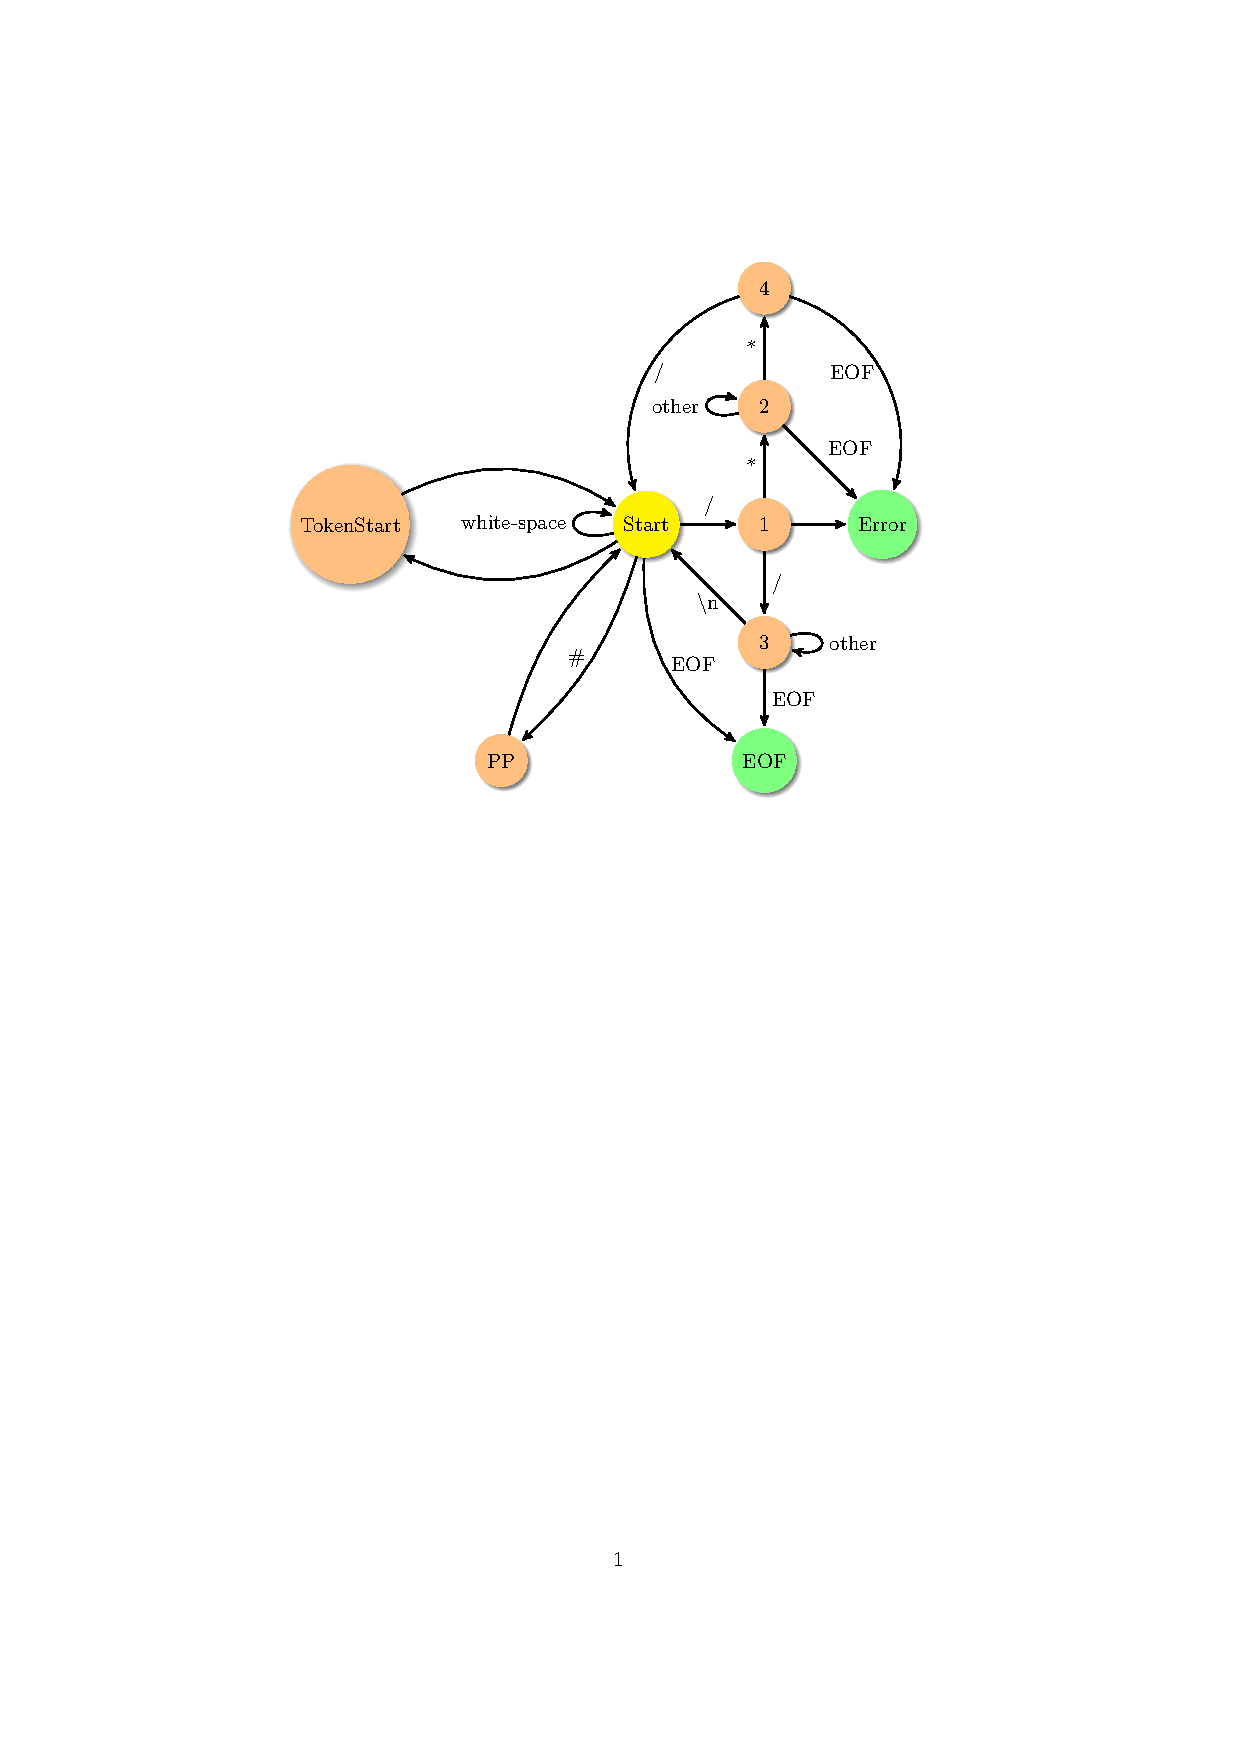
\includegraphics{ifacegen-automata.pdf}
%
%\begin{grammar}
%[(colon){ ::$\Rightarrow$ }]
%[(semicolon){ $|$}]
%[(comma){}]
%[(period){\\}]
%[(quote){\begin{bf}}{\end{bf}}]
%[(nonterminal){$\langle$}{$\rangle$}]
%<API header> : $\epsilon$; <declaration>, <API header>.
%<declaration>: <type spec>, <function or struct decl>.
%<function or struct decl>: identifier, <function declaration>; "\{", <struct declaration>.
%<expression>:<number>;\\
%<number>, <relational operator>, <number>.
%<number>:<digit>;<digit>,<number>.
%<digit>:"0";"1";"2";"3";"4";"5";"6";"7";"8";"9".
%<relational operator>:"$=$";"$\lessthan\greaterthan$";
%"$\lessthan$";"$\greaterthan$";
%"$\lessthan=$";"$\greaterthan=$";"in".
%\end{grammar}

